\title{LEZIONE 12 19/05/2020}\newline
\textbf{link} \href{https://web.microsoftstream.com/video/4108da02-d3de-45e4-ab46-94d93c315e97}{clicca qui}
\section{Dinamica della macchina a 1 grado di libertà (MTU)}
La \textbf{macchina} è un sistema meccanico che utilizza energià diversa dall'energia meccanica, per compiere del lavoro.\newline
\newline
Per modellare una macchina è sempre possibile suddividere la macchina nei componenti che la compongono:
\begin{itemize}
    \item \textbf{Motore}: sfrutta energia differente da quella meccanica, per produrre energia che viene resa disponibile alla macchina.
    \item \textbf{Trasmissione}: collega motore e utilizzatore, creando un rapporto fra la velocità del motore e dell'utilizzatore, detto \textbf{rapporto di trasmissione}.
    \item \textbf{Utilizzatore}: impiega la potenza meccanica prodotta dal motore per compiere del lavoro utile.
\end{itemize}
In questo corso studieremo sempre macchiana a un grado di libertà, nel senso che ci basterà sempre e soltanto una coordinata per descrivere tutti i componenti:\newline
[immagine dagli appunti del prof]
\begin{center}
    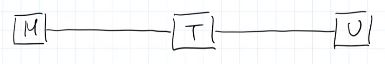
\includegraphics[height=2cm]{../lezione12/img1.JPG}
\end{center}
Solitamente la coordinata scelta è la velocità angolare $\omega_m$ della macchina.\newline
\newline
La dinamica della macchina MTU viene studiata tramite il teorema dell'energia cinetica.\newline
\newline
L'elemento che dissipa potenza è la trasmissione, per questo dovremo scrivere i teoremi sotto l'ipotesi di vincoli non perfetti, cioè con attrito.\newline
\newline
Il teorema dell'energia cinetica ci dice che la somma della potenza di tutte le forze e coppie attive e di quella dissipata per attrito è ugule alla derivata rispetto al tempo dell'energia cinetica di tutto il sistema:
\[
    W + W_d = \frac{dE_c}{dt}
\]
Ci risulta però comodo scomporre questi termini per i tre componenti della macchina MTU:
\[
    W_m + W_u + W_p = \frac{dE_c}{dt}
\]
con $W_m$ potenza motrice, con $W_u$ potenza dell'utilizzatore e $W_p$ potenza dissipata nella trasmissione (persa per attrito).\newline
\newline
Tutti questi termini sono dotati di segno, l'unico conosciuto è che $W_p <0$, gli altri possono essere positivi o negativi a seconda delle condizioni di funzionamento della macchina.\newline
\newline
Anche l'energia cinetica può essere scomposta per le tre componenti, tuttavia considereremo sempre trascurabile l'inerzia associata a tutti gli organi che si trovano all'interno della trasmissione, quindi si può trascurare la sua energia cinetica:
\[
    E_c = E_{cm} + E_{cu} + \cancel{E_{cr}} = E_{cm} + E_{cu}
\]
con $E_{cm}$ energia cinetica del motore e $E_{cu}$ energia  cinetica dell'utilizzatore.\newline
\newline
\subsection{Motore}
In questo corso considereremo due tipologie di motori:
\begin{itemize}
    \item \textbf{Motori a combustione interna}
    \item \textbf{Motori elettrici}:
    \begin{itemize}
        \item \textbf{a corrente continua (DC)}
        \item \textbf{a corrente alternata (AC)}
    \end{itemize}
\end{itemize}
\ \newline
Per semplificare la trattazione sui motori studiamo la sola coppia equivalente ridotta all'albero motore che produca la stessa potenza di tutte le forze e coppie di tutti i componenti:
\[
    M_m^* = \text{coppia ridotta all'albero motore}\; \rightarrow  W_m = \vec{M}_m^* \;\text{x}\;\vec{\omega}_m = \sum_i \vec{F}_i \;\text{x}\;\vec{v}_i + \sum_j \vec{C}_j \;\text{x}\;\vec{\omega}_j
\]
Riscriviamo ora la potenza con i Jacobiani del moto, che legano la velocità di qualsiasi punto e la velocità angolare di qualsiasi corpo con la coordinata indipendente, cioè la velocità angolare del motore
\[
    W_m = \left(\sum_i \vec{F}_i \;\text{x}\; \frac{d \vec{P}_i}{d \theta_m} + \sum_j \vec{C}_j \;\text{x}\;\frac{d \vec{\theta}_j}{s \theta_m} \right) \omega_m = \vec{M}_m \;\text{x}\;\vec{\omega}_m
\]
dove il termine $M_m^* = \sum_i \vec{F}_i \;\text{x}\; \frac{d \vec{P}_i}{d \theta_m}$ rappresenta la coppia ridotta all'albero motore e i termini $\frac{d \vec{P}_i}{d \theta_m}$ e $\frac{d \vec{\theta}_j}{s \theta_m}$ sono i Jacobiani del moto.\newline
\newline
Analogamente, possiamo fare un discorso del tutto simile per l'energia cinetica, cioè è più facile considerare un'inerzia equivalente a tutte le inerzie che si trovano a monte della trasmissione:
\[
    J_m^* = \text{momento dìinerzia ridotto all'albero motore}\;
\]
\[
    E_{cm} = \frac{1}{2} J_m^* \omega_m^2 = \frac{1}{2}\sum_{i=1}^{n_{cm}}\left( m_i v_{Gi}^2 + J_{Gi} \omega_i^2 \right)
\]
con $n_{cm}$ numero di corpi rigidi presenti a lato motore.\newline
Siccome il sistema è a un grado di libertà possiamo riscrivere l'energia cinetica sfruttando gli Jacobiani del moto:
\[
    E_{cm} = \frac{1}{2} \sum_{i=1}^{n_{cm}} \left( m_i \Lambda_{Gi}^2 + J_{Gi} \Lambda_{\omega i}^2 \right) = \frac{1}{2} J_m^* \omega_m^2
\]
dove $J_m^* = m_i \Lambda_{Gi}^2 + J_{Gi} \Lambda_{\omega i}^2$ e le due $\Lambda$ rappresentano gli Jacobiani del moto, ovvero la derivata dello spostamento del baricentro e della rotazione del corpo i-esimo rispetto alla coordinata indipendente $\theta_m$.\newline
\newline
Una volta fatte le riduzioni equivalenti per gli alberi motori possiamo interpretare le macchina a un grado di libertà come segue:\newline
[immagine dagli appunti del prof]
\begin{center}
    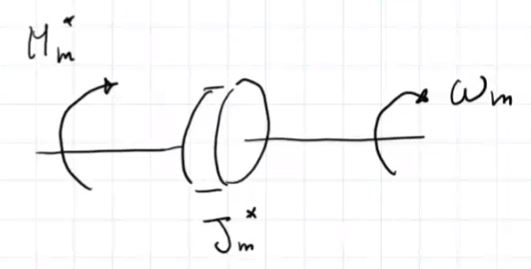
\includegraphics[height=3cm]{../lezione12/img2.JPG}
\end{center}
Indipendentemente dalla tipologia di motore considerato, il modello che ne facciamo è quello di avere un albero che ruota alla velocità $\omega_m$, su cui è applicata la coppia $M_m^*$ ridotta all'abero motore, e su questo albero è calettato (rigidamente collegato) un'inerzia, detta \textbf{volano}, pari a $J_m^*$.\newline
\newline
Ricordiamo che $M_m^* = M_m^*(\omega_m)$, e nei casi di \textbf{macchine a regime periodico} possiamo dire che  $M_m^* = M_m^*(\omega_m, \theta_m)$.\newline
\newline
La funzione $M_m^* = M_m^*(\omega_m)$ definisce una \textbf{curva caratteristica}.\newline
Ogni punto della curva caratteristica di un motore rappresenta una \textbf{condizione di regime}, cioè ogni punto della curva è calcolato considerando un $\omega_m$ costante. Ma se $\omega_m$ è costante, allora anche l'energia cinetica è costante, cioè la sua derivata è nulla.\newline
\newline
Vediamo qualche esempio.
\subsubsection{Motore a combustione interna}
[immagine dagli appunti del prof]
\begin{center}
    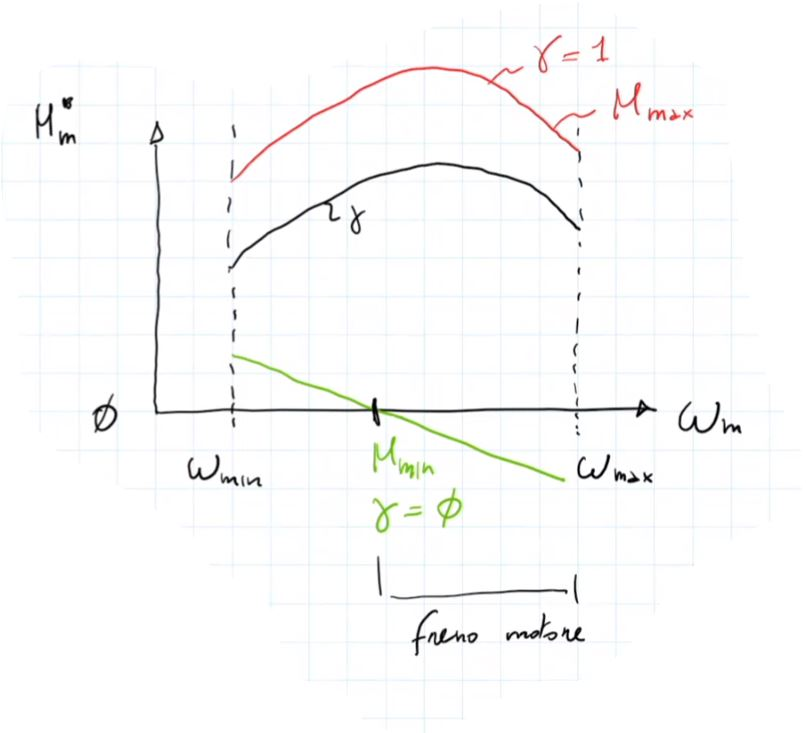
\includegraphics[height=3cm]{../lezione12/img3.JPG}
\end{center}
I valori $\omega_{min}$ e $\omega_{max}$ sono valori delimitanti oltre i quali il motore si spegne o va in "fuori giro".\newline
\newline
Il grafico è approssimabile a una parabola.\newline
\newline
Il \textbf{grado di ammissione} $\gamma$ (quanto schiaccio sul pedale dell'accelleratore), che varia fra $0 \leq \gamma \leq 1$, mi determina la forma della curva caratteristica.\newline
\newline
Dove la curva è negativa, il motore si comporta da freno.\newline
\newline
Per ogni valore di $\gamma$ diverso da $0$ o $1$, per trovare la forma delal curva caratteristica, posso fare una media pesata:
\[
    M_m^* (\bar{\omega}_m) = \gamma M_max(\bar{\omega}_m) + (1- \gamma) M_{min} (\bar{\omega}_m)
\]
\subsubsection{Motori elettrici in corrente continua}
[immagine dagli appunti del prof]
\begin{center}
    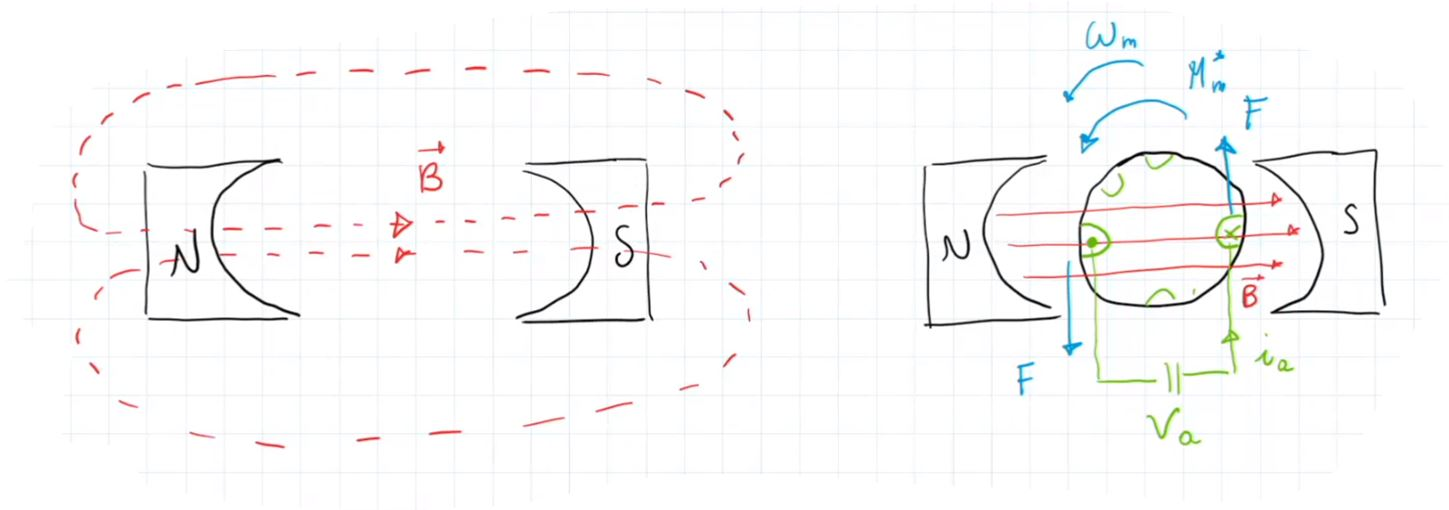
\includegraphics[height=3cm]{../lezione12/img4.JPG}
\end{center}
I motori elettrici sono caratterizzati da un campo magnetico $\vec{B}$, approssimabili con delle lettere fra i componenti $N$ e $S$, che rappresentano lo \textbf{statore}.\newline
\newline
All'interno è posto un \textbf{rotore}, che è il nostro albero motore. Il rotore contiene degli avvolgimenti di circuiti elettrici (in verde) per cui si manifestano delle forze di Lorentz (in blu), che generano una coppia che mette in rotazione l'albero motore.\newline
\newline
In condizione di regime ($\omega_m =$ costante) le equazioni che rappresentano il motore sono:
\[
    V_a = R i_a + e
\]
con $e$ \textbf{forza elettromotrice}
\[
    e = K_{\phi} \omega_m
\]
La legge di Lorentz ci permette di determinare la coppia motrice:
\[
    M_m^* = K_{\phi} i_a = \frac{K_{\phi} V_a - K_{\phi}^2 \omega_m}{R}
\]
che è l'equazione di una retta:\newline
[immagine dagli appunti del prof]
\begin{center}
    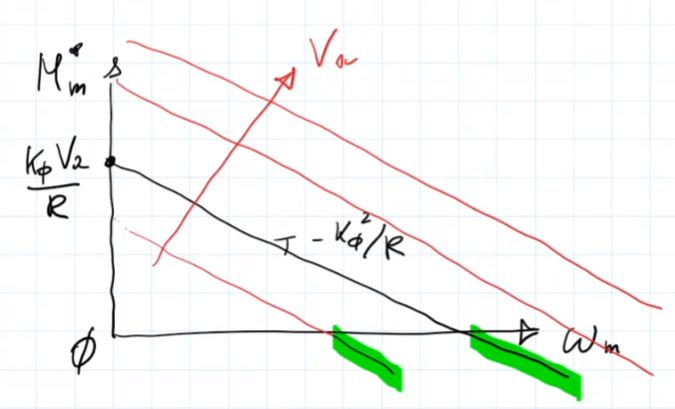
\includegraphics[height=3cm]{../lezione12/img5.JPG}
\end{center}
in cui modificando $V_a$ posso alzare la quota della retta.
\subsubsection{Motori elettrici in corrente alternata}
Anche questi motori sono composti da \textbf{rotore} e \textbf{statore}:\newline
[immagine dagli appunti del prof]
\begin{center}
    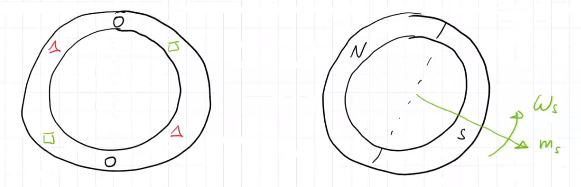
\includegraphics[height=3cm]{../lezione12/img6.JPG}
\end{center}
Lo statore è un circuito trifase (cerchiolino, quadratino e triangolino) che crea un campo magnetico rotante con velocità angolare pari a $\omega_s$, che prende il nome di \textbf{velocità di sincronismo}:
\[
    \omega_s = \frac{2 \pi f_a}{p}
\]
con $f_a$ \textbf{frequenza di alimentazione} (in Europa $50Hz$) e $p$ è il \textbf{numero di poli} (per noi $1$).\newline
\newline
All'interno dell ostatore ci sta un rotore, che altro non è che l'albero motore:\newline
[immagine dagli appunti del prof]
\begin{center}
    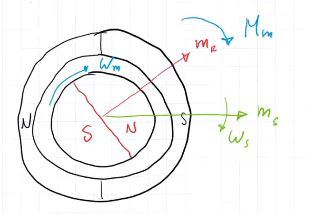
\includegraphics[height=3cm]{../lezione12/img7.JPG}
\end{center}
Il rotore crea un campo magnetico $m_R$, che crea una coppia $M_m$ che cerca di far allineare il campo magnetico $m_R$ con quello $m_S$.\newline
\newline
La curva caratteristica del motore in corrente alternata è:\newline
[immagine dagli appunti del prof]
\begin{center}
    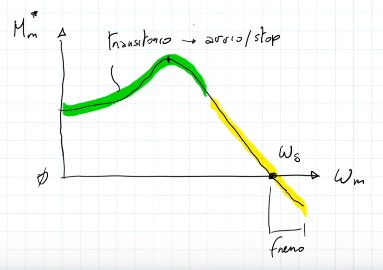
\includegraphics[height=3cm]{../lezione12/img8.JPG}
\end{center}
Perchè il motore funzioni correttamente si vuole sempre lavorare in vicinanza della velocità $\omega_s$ (in giallo), la zona in verde, invece, viene percorsa solo in caso di avvio o stop del motore.\newline
\newline
Notiamo come il motore in corrente alternata (in procinto di $\omega_s$, cioè a regime operativo) si comporta allo stesso modo del motore in corrente continua.
\subsection{Utilizzatore}
[immagine dagli appunti del prof]
\begin{center}
    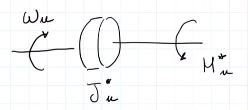
\includegraphics[height=3cm]{../lezione12/img9.JPG}
\end{center}
Tutto il discorso fatto per il motore si può riflettere sull'utilizzatore, introducendo quindi un \textbf{momento ridotto all'albero utilizzatore} $M_u^*$ alla quale corrisponde una potenza:
\[
    W_u = M_u^* \omega_u = \sum \vec{F}_i \;\text{x}\; \vec{v}_i + \sum \vec{C}_j + \vec{\omega}_j
\]
Allo stesso modo si introduce un \textbf{momento di inerzia ridotto all'albero utilizzatore} $J_u^*$, al quale corrisponde un energia cinetica:
\[
    E_{cu} = \frac{1}{2} J_u^* \omega_u^2
\]
\ \newline
Nel corso vedremo tre tipologie di utilizzatori:
\begin{itemize}
    \item \textbf{Coppia costante} (per esempio tutti i \textbf{sollevatori}) indipendentemente dalla velocità dell'utilizzatore: $M_u^* = - M_{uo}$.\newline
    [immagine dagli appunti del prof]
    \begin{center}
        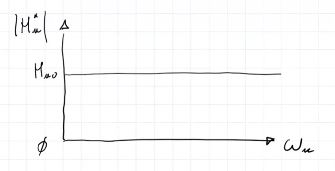
\includegraphics[height=2cm]{../lezione12/img10.JPG}
    \end{center}
    \item \textbf{Parabola centrata nell'origine} (per tutti i casi in cui è presente della fluidodinamica): $M_u^* = - k \omega_u^2$.\newline
    [immagine dagli appunti del prof]
    \begin{center}
        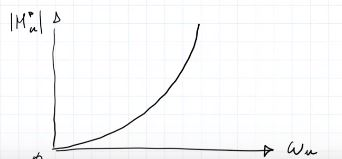
\includegraphics[height=2cm]{../lezione12/img11.JPG}
    \end{center}
    \item \textbf{somma delle due precedenti}: $M_u^* = - (M_{uo} + k \omega_u^2)$\newline
    [immagine dagli appunti del prof]
    \begin{center}
        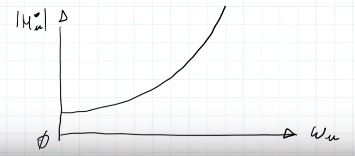
\includegraphics[height=2cm]{../lezione12/img12.JPG}
    \end{center}
\end{itemize}